\newpage
\begin{center}
    {\large \textbf{Functions of Bounded Variation}}
\end{center}

\vs

\dfn Let $F:\R\ra \C$ and fix $x\in \R$. We define $T_F:\R\ra [0, \infty]$ by
\[T_F(x) = \sup\left\{\sum_{j = 1}^n |F(x_j) - F(x_{j - 1})| \ :\ n\in \N,\ x_0 < x_1< \cdots <x_n = x\right\}\]
We say that $F$ is of bounded variation on $\R$ if $T_F(x) < \infty$ for all $x\in \R$. If $F:[a,b]\ra \C$ we define $T_{F,a}(x)$ the same way but with $x_0 = a$ and $x \leq b$. We say that $F$ is of BV on $[a,b]$ if $T_{F,a}(x) < \infty$ for all $a \leq x\leq b$.

\vs 

\textbf{Theorem} (Lebesgue 1904) If $F\in BV$, $F\in BV[a,b]$, then $F\p(x)$ exists a.e. on $\R$.

\vs

\textbf{Example:} Let 
\[F(x) = \begin{cases} x\cos\lp\frac{1}{x}\rp & 0 < x \leq \frac{2}{\pi}\\ 0 & o.w.\end{cases}\]
There is no bounded variation of this function. For $k\in \N$ let
\[\PP_k = \left\{0, \frac{2}{\pi(2k)}, \frac{2}{\pi(2k - 1},\ldots, \frac{2}{\pi 2}. \frac{2}{\pi}\right\}\]
be the partition that we choose of $[0, 2/\pi]$. Then we have that
\begin{align*}
    T_{F, 0}\lp\frac{2}{\pi}\rp \geq 
    \sum_{j = 1}^2k | F(x_j) - F(x_{j - 1})|
\end{align*}

\vs

\setcounter{thm}{26}

\begin{thm}
Let $F$ be a function
\begin{enumerate}
    \item $F\in BV$ iff $\Re(F)$ and $\Im(F)$ are $BV$
    \item $F\in BV$ iff $F = F_1 - F_2$ where $F_1$ and $F_2$ are bounded and monotone
    \item IF $F\in BV$, $F(x+) = \lim_{y \ra x^+} F(y)$ and $F(x-)$ exist for all $x\in \R$.
    \item If $F\in BV$ the set of points where $F$ is not continuous is countable.
    \item If $F\in BV$, set the $G(x) = F(x+)$ for all $x\in \R$. Then $G(x) = F(x)$ a.e. and $G\p(x),\ F\p(x)$ exist and are equal a.e.
\end{enumerate}
\end{thm}

\vs

\textbf{Lemma} If $F\in BV[a,b]$ then $F$ is bounded.

\vs

\textbf{Lemma} If $F:[a,b]\ra \R$, $F\in BV[a,b]$. If $a \leq c < d \leq b$. Then 
\[T_{F, a}(c) \leq T_{F_a}(d)\]

\vs

\textbf{Lemma} If $F\in BV[a,b]$ and $a\leq c < d \leq b$, then $F\in BV[a,c]$ and $F\in BV[c,d]$ and
\[T_{F, a}(d) = T_{F, a}(c) + T_{F, c}(d).\]

\vs

\textbf{Proposition} Let $F\in BV[a,b]$. Then $G = F_1 - F_2$ where $F_1$ and $F_2$ are monotone increasing on $[a,b]$.


\vs

\dfn Let $E\subset \R$. Let $\mathfrak{I}$ be a collection of intervals in $\R$. We say that $\mathfrak{I}$ is a \textbf{\textit{Vitali cover}} for $E$ if for every $x\in E$ and for every $\vep > 0$ there is some $I\in \mathfrak{I}$ such that $x\in I$ and $\ell(I) < \vep$.

\vs

\textbf{Lemma} (Vitali Covering Lemma) Let $E\subset \R$ and suppose $m^*(E) < 0$. Suppose $\mathfrak{I}$ is a collection of closed and bounded intervals of $\R$ that form a Vitali cover for $E$. Then for every $\vep > 0$ there are intervals $I_1, I_2, \ldots, I_n \in \mathfrak{I}$ such that $I_i\cap I_j = \es$ and $m^*\lp E\backslash \bigcup_{k = 1}^n I_k \rp < \vep$.

\vs

\dfn We define the \textbf{\textit{Dini Derivates}} of $f$ at $x$ is given as follows
\begin{align*}
    D^+f(x) &= \limsup_{h \ra 0^+} \frac{f(x + h) - f(x)}{h},\\
    D^-f(x) &= \limsup_{h \ra 0^-} \frac{f(x + h) - f(x)}{h},\\
    D_+f(x) &= \liminf_{h \ra 0^+} \frac{f(x + h) - f(x)}{h},\\
    D_-f(x) &= \liminf_{h \ra 0^-} \frac{f(x + h) - f(x)}{h}.
\end{align*}


\vs

\textbf{Lemma:} If $F\in BV$ is real-valued, then $T_F + F$ and $T_F - F$ are increasing. Moreover
\[F = \frac{1}{2}(T_f + F) + \frac{1}{2}(T_F - F)\]
this is called the \textbf{\textit{Jordan decomposition}} of $F$

\vs

\dfn We define the set of \textbf{\textit{Normalized Bounded Variation}} functions $NBV\seq BV$ by \[NBV = \{F\in BV\ :\ F\text{ is right continuous and }F(-\infty = 0\}.\]

\vs

\textbf{Theorem:} Let $F:[a,b] \ra \R$ be a monotone increasing function. Then the derivative $F\p$ exists almost everywhere, and $F\in L^1([a,b])$, and 
\[\int_a^b F\p(x)\ dx = F(b) - F(a).\]

\vs

\dfn We say that a function $F:\R\ra \C$ is \textbf{\textit{absolutely continuous}} if for every $\vep > 0$ there exists a $\de > 0$ such that for any finite set of disjoint intervals $(a_1,b_1),\ldots,(a_N,b_N)$,
\[\sum_1^N(b_j - a_j) < \de\quad \Longrightarrow \quad\sum_1^N|F(b_j)- F(a_j)| < \vep\]

\textbf{Lemma:} Let $F:[a,b]\ra \R$ be monotone increasing and $AC$ on $[a,b]$. Then the Borel measure $\nu_F$ on $([a,b], \B_\R)$ defined by 
\[\nu_F((c, d]) = F(d) - F(c)\]
is absolutely continuous with respect to $m$ on $[a,b]$.

\vs

\textbf{Corollary:} If $F$ is $\nearrow$ and $F\in AC$ on $[a,b]$ then there is an $F\in L^1([a,b]) \cap L^+$ such that 
\[F(x) = \int_1^x f(t)\ dt + F(a)\]
for all $x\in [a,b]$.

\vs

\textbf{Corollary:} If $F\in AC([a,b])$, then there is a $f\in L^1([a,b])$ such that 
\[F(x) - F(a) = \int_a^x f(t)\ dt.\]

\vs

\setcounter{thm}{34}

\begin{thm}
Let $F:[a,b] \ra \R$. Then TFAE
\begin{enumerate}[\hspace{1em}(a)]
    \item $F$ is $AC$ on $[a,b]$.
    \item $F(x) - F(a) = \int_a^x f(t)\ dt$ for some $f\in L^1([a,b])$.
    \item $F$ is differentiable a.e. on $[a,b]$, $F\p \in L^1([a,b], m)$, and $F(x) - F(a) = \int_a^x F\p(t)\ dt$.
\end{enumerate}
\end{thm}

Note: go over the proof of $(b)\Ra (c)$ in Folland


\vs


\dfn Let $F:{a,b}\ra \R$. We say that $F$ is \textbf{\textit{Lipschitz}} if there is some $M > 0$ such that $|F(x) - F(y)| \leq M|x - y|$ for all $x,y\in [a,b]$.

\textbf{Exercises:}
\begin{enumerate}
    \item If $F$ is Lipschitz then F is $AC([a,b])$.
    \item If $F$ is differentiable at all $x\in [a,b]$, and $|F\p(x)|\leq M$ then $F$ is Lipschitz $\Ra$ F is in $AC([a,b])$.
\end{enumerate}

\vs

\dfn Let $\vphi:(a,b)\ra \R$. We say that $\vphi$ is \textbf{\textit{convex}} if for all $x,y\in (a,b)$, and for all $\lambda \in [0,1]$, 
\[\vphi(\lambda x + (1-\lambda)y)\leq \lambda \vphi(x) + (1-\lambda)\vphi(y).\]

\vs


\textbf{Proposition.} Let $\vphi:(a,b)\ra \R$ and suppose $\vphi^{\prime\prime}(X)$ exists for all $x\in (a,b)$. Then the following are equivalent:
\begin{enumerate}[\hspace{1em} (i)]
    \item $\vphi$ is convex on $(a,b)$
    \item $\vphi(y) \geq \vphi(x) + \vphi\p(x) (y - x)$ for all $x,y \in (a,b)$.
    \item $\vphi^{\prime\prime}(x) \geq 0$ for all $x\in (a,b)$
\end{enumerate}

\vs

\textbf{Chordal Slope Lemma:} Let $\vphi:(a,b) \ra \R$ be a convex function. Suppose $x, x\p, y, y\p\in (a,b)$ with $x \leq x\p < y$ and $x < y \leq y\p$. Then 
\[\frac{\vphi(y) - \vphi(x)}{y - x}\leq \frac{\vphi(y\p) - \vphi(x\p)}{y\p - x\p}\]

\begin{center}
    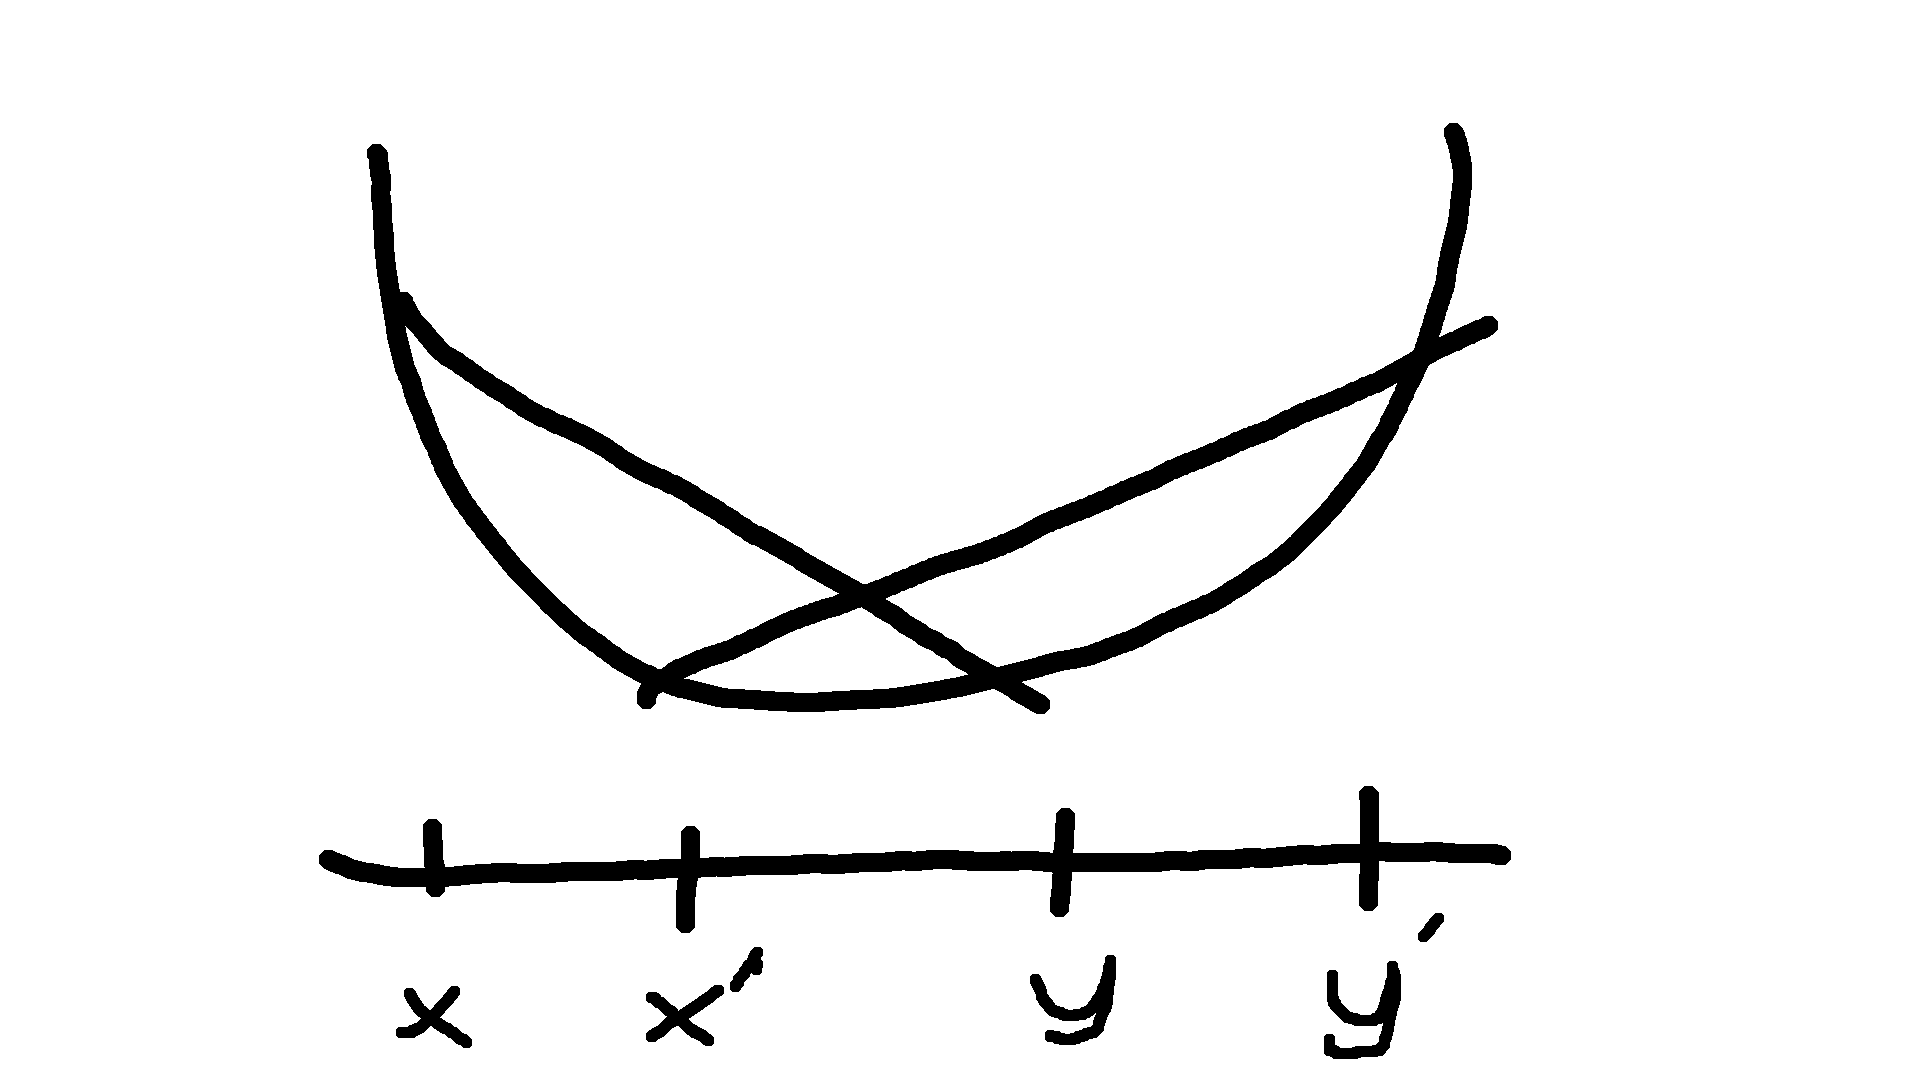
\includegraphics[scale = 0.5]{chordal.png}
\end{center}

\vs

\textbf{Corollary,} If $x_1 < x_2 \leq x_3 < x_4$ for a convex function $\vphi$ then
\[\frac{\vphi(x_2) - \vphi(x_1)}{x_2 - x_1}\leq \frac{\vphi(x_4) - \vphi(x_3)}{x_4 - x_3}\]

\vs

\textbf{Theorem.} If $\vphi:(a,b) \ra \R$ is convex, then $\vphi$ is $AC$ on every closed sub-interval $[c,d]\subset (a,b)$. Moreover,
\[\lim_{h\ra 0^+} = \frac{\vphi(x + h) - \vphi(x)}{h} = \vphi\p_R(x+)\]
and 
\[\lim_{h\ra 0^-} = \frac{\vphi(x + h) - \vphi(x)}{h} = \vphi\p_L(x-)\]
exist at every $x$, and this will imply $\vphi\p$ exists except at a countable number of points in $(a,b)$.

\vs

\textbf{Jensen's Inequality.} Suppose $\vphi:\R\ra \R$ be convex. Let $f:[0,1]\ra \R$ be Lebesgue integrable on $[0,1]$ so that 
\[\int_{[0,1]}|f|\ dm < \infty.\]
Suppose also that $\vphi \circ f:[0,1]\ra \R$ is Lebesgue integrable over $[0,1]$. Then 
\[\vphi\lp\int_{[0,1]} f(x)\ dx\rp \leq \int_{[0,1]}(\vphi\circ f)(x)\ dx.\]